\documentclass[11pt, a4paper]{article}
\usepackage[letterpaper, portrait, margin=0.5in]{geometry}
\usepackage[english]{babel}  % force American English hyphenation patterns
\usepackage{amsmath,mathtools}

\usepackage{graphicx}
\usepackage{wrapfig}


\begin{document}
\title{Chapter 21 Electric Charge And Electric Field}
\author{Apostolos Delis}
\date{\today}
\maketitle

\tableofcontents
\section[21.1, Electric Charge]{Electric Charge}
Electrostatics: the interactions between electric charges that are at rest
\subsection{Electric Charge and The Structure of Matter}
\begin{itemize}
    \item The structure of atoms can be described in terms of three particles: the
        negatively charged electron, the positively charged proton, and the uncharged
        neutron
    \item The protons and neutrons in an atom make up a small, very dense core called the
        nucleus
    \item Note that the masses of the proton and neutron are nearly equal and are roughly
        2000 times the mass of the electron.
    \item The negative charge of the electron has exactly the same magnitude as the
        positive charge of the proton.
    \item The number of protons or electrons in a neutral atom of an element is called
        the atomic number of the element.
    \item A negative ion is an atom that has gained one or more electrons. This gain or
        loss of electrons is called ionization.
\end{itemize}
\subsection{Electric Charge is Conserved}
\begin{itemize}
    \item Principle of Conservation of Charge: The algebraic sum of all the electric
        charges in any closed system is constant.
    \item The second important principle is: The magnitude of charge of the electron
        or proton is a natural unit of charge.
    \item Every observable amount of electric charge is always an integer multiple of this
        basic unit. We say that charge is quantized. Charge can't be divided more than
        one electron or proton.
\end{itemize}
\section[21.2, Conductors, Insulators, And Induced Charges]{Conductors, Insulators, And
    Induced Charges}
\begin{itemize}
    \item Conductors permit the easy movement of charge through them, while insulators do
        not
    \item Most metals are good conductors, while most nonmetals are insulators
    \item Some materials called semiconductors are intermediate in their properties
        between good conductors and good insulators.
\end{itemize}
\subsection{Charging By Induction}
\begin{itemize}
    \item We can charge a metal ball using a copper wire and an elextrically charged
        plastic rod, however this requires giving off some excess electrons
    \item Charging by induction lets the plastic rod give another body a charge of
        opposite sign without losing any of its own charge
\end{itemize}
\subsection{Electric Forces On Uncharged Objects}
\begin{itemize}
    \item  A charged body can exert forces even on objects that are not charged themselves
    \item Polarization: all the positive charge in an object goes to one side, all the
        negative goes to the other
\end{itemize}
\section[21.3, Coulomb's Law]{Coulomb's Law}
\begin{itemize}
    \item The magnitude of the electric force between two point charges is directly
        proportional to the product of the charges and inversely proportional to the
        square of the distance between them
    \item The magnitude $F$ of the force of two point charges $q_1$ and $q_2$ that are a
        distance $r$ from each other can be expressed as
        \begin{equation}
            F = \frac{1}{4\pi\epsilon_0}\frac{|q_1 q_2|}{r^2}
        \end{equation}
    \item Thus, this force is similar to the force of gravity between two objects
\end{itemize}
\subsection{Fundamental Electric Constants}
\begin{itemize}
    \item The SI electric units include most of the familiar units such as the volt, the
        ampere, the ohm, and the watt.
    \item The SI unit of electric charge is called one coulomb (1 C), in coloumbs, we
        have that
        \begin{equation}
            k = \frac{1}{4\pi\epsilon_0} = 8.987551787 \times 10^9 N\cdot m^2 / C^2
        \end{equation}
    \item This value will often just get approximated to $9.0\times 10^9 N \cdot m^2 /C^2$
\end{itemize}
\subsection{Superposition of Forces}
Experiments show that when two charges exert forces simultaneously on a third charge, the
total force acting on that charge is the vector sum of the forces that the two charges
would exert individually. This phenomena is known as the superposition of forces
\section[21.4, Electric Field and Electric Forces]{Electric Field and Electric Forces}
\subsection{Electric Field}
\begin{itemize}
    \item An electric field is a force similar to gravity in that it does not need to
        physically contact an object and can simply act across empty space
    \item The electric force on a charged body is exerted by the electric field created by
        other charged bodies.
    \item The electric field at a certain point is equal to the electric force per unit
        charge experienced by a charge at that point:
        \begin{equation}
            \vec{\mathbf{E}} = \frac{\vec{\mathbf{F_0}}}{q_0}
        \end{equation}
    \item So in this equation, $\vec{\mathbf{F_0}}$ is the Electric force at the test
        charge $q_0$, while $\mathbf{\vec{E}}$ is in terms of electric force per unit
        charge
\end{itemize}
\subsection{Electric Field of a Point Charge}
\begin{itemize}
    \item We call the location of the charge the source point, and we call the point P
        where we are determining the field the field point.
    \item It also often useful to introduce $\hat{r}$, a unit vector that points along
        the line from the source point to the field point
    \item Take the displacement vector $\vec{\mathbf{r}}$ and divide by the distance
        $|r|$, so then $\hat{\mathbf{r}} = \vec{\mathbf{r}} / |r|$
    \item The magnitude $E$ of the electric field at $P$ is:
        \begin{equation}
            E = \frac{1}{4\pi\epsilon_0}\frac{|q|}{r^2}
        \end{equation}
    \item Using the unit vector $\hat{\mathbf{r}}$, we can write a vector equation that
        gives both magnitude and direction of the electric field
        \begin{equation}
            \vec{\mathbf{E}} = \frac{1}{4\pi\epsilon_0}\frac{q}{r^2}\hat{\mathbf{r}}
        \end{equation}
\end{itemize}
\section[21.5 Electric-Field Calculations]{Electric-Field Calculations}
\subsection{The Superposition of Electric Fields}
\begin{itemize}
    \item The total force $\vec{\mathbf{F_0}}$ that the charge distribution exerts on
        $q_0$ is the vector sum of the total forces
        \begin{equation}
            \vec{\mathbf{F_0}} = \vec{\mathbf{F_1}} + \vec{\mathbf{F_2}} + ... =
            q_0 \vec{\mathbf{E_1}} + q_0 \vec{\mathbf{E_1}} + ...
        \end{equation}
    \item The combined effect of all the charges in the distribution is described by the total
        electric field $\vec{\mathbf{E}}$ at point $P$
        \begin{equation}
            \vec{\mathbf{E}} = \frac{\vec{\mathbf{F_0}}}{q_0} =
            \vec{\mathbf{E_1}} + \vec{\mathbf{E_2}} + ...
        \end{equation}
    \item The total electric field at P is the vector sum of the fields at P due to each
        point charge in the charge distribution, this is the principle of superposition of
        electric fields.
    \item When charge is distributed along a line, over a surface, or through a volume,
        we also want the charge density of the medium
\end{itemize}
\section[21.6 Electric Field Lines]{Electric Field Lines}
\begin{itemize}
    \item An electric field line is an imaginary line or curve drawn through a region of space
        so that its tangent at any point is in the direction of the electric-field vector at
        that point.
    \item Electric field lines show the direction of $\vec{\mathbf{E}}$ at each point, and their spacing
        gives a general idea of the magnitude of $\vec{\mathbf{E}}$ at each point
    \item Electric field lines for three different charge distributions. In general, the
        magnitude of $\vec{\mathbf{E}}$ is different at different points along a given field line

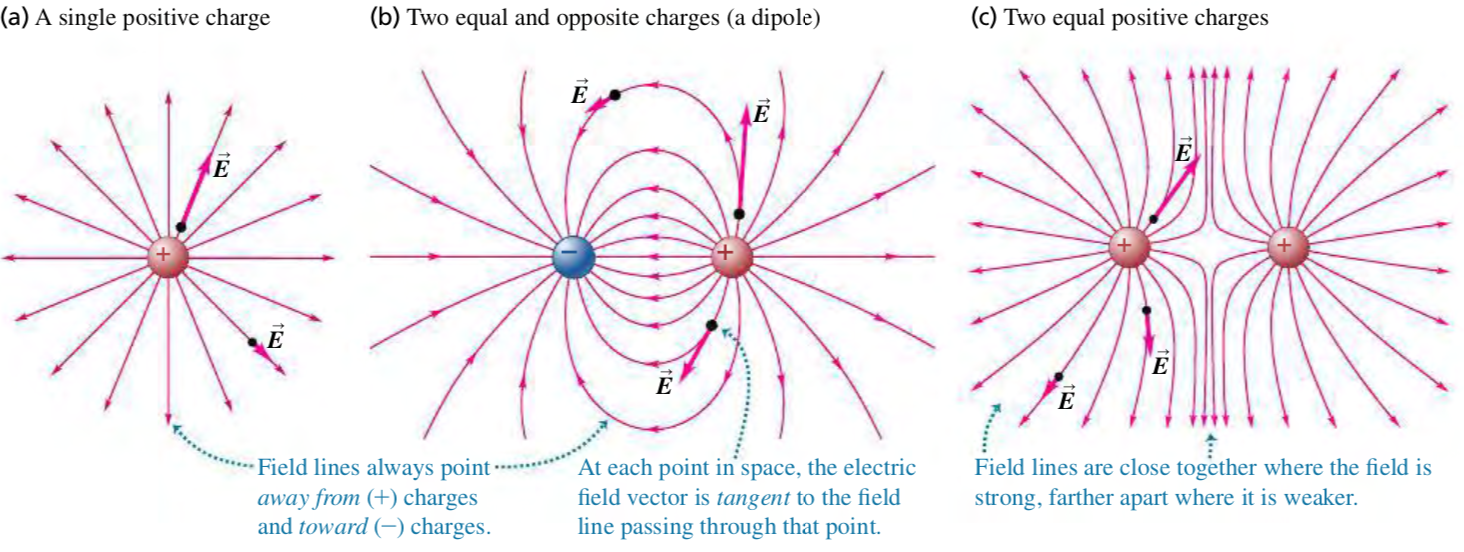
\includegraphics[scale=0.50]{images/E_charge_distributions.png}
\end{itemize}
\section[21.7, Electric Dipoles]{Electric Dipoles}
An electric dipole is a pair of point charges with equal magnitude and opposite
sign seperated by a distance $d$
\subsection{Force and Torque on an Electric Dipole}
\begin{itemize}
    \item To begin, place an electric dipole in a uniform external electric field
        $\vec{\mathbf{E}}$. Both forces $\vec{\mathbf{F_+}}, \vec{\mathbf{F_-}}$ on the two
        charges have magnitude $qE$
    \item The magnitude of the net torque is twice the magnitude of the individual
        torques
        \begin{equation}
            \tau = (qE)(d\sin\phi)
        \end{equation}
    \item Where $d\sin\phi$ is the perpendicular distance between the lines of action of
        the two forces
    \item The product of charge $q$ and distance $d$ is the magnitude of a quantity known
        as the electric dipole moment, denoted $p = qd$
    \item In terms of vector torque on the electric dipole, we can write the vector form:
        \begin{equation}
            \vec{\mathbf{\tau}} = \vec{\mathbf{p}} \times \vec{\mathbf{E}}
        \end{equation}
    \item Torque is thus greatest when $\vec{\mathbf{p}}$ and $\vec{\mathbf{E}}$ are
        perpendicular and is zero when they are parallel or antiparallel
\end{itemize}
\subsection{Potential Energy Of An Electric Dipole}
\begin{itemize}
    \item When a dipole changes direction in an electric field, the electric-field torque
        does work on it
    \item The work $dW$ done by a torque $\tau$ during an infinitesimal displacement
        $d\phi$ is given by $dW = \tau d\phi$ Because torque is in the direction of
        decreasing $\phi$, we must have that $\tau = -pE\sin\phi$ and
        \begin{equation}
            dW = \tau d\phi = -pE\sin\phi d\phi
        \end{equation}
    \item So the total work done from $\phi_1$ to $\phi_2$ is given by
        \begin{equation}
            W= \int_{\phi_1}^{\phi_2} (-pE\sin\phi)d\phi = pE(\cos\phi_2 - \cos\phi_1)
        \end{equation}
    \item Work is the negative change of potential energy, so work is $W = U_1 - U_2$, so
        then we have the equation of potential energy:
        \begin{equation}
            U(\phi) = -pE\cos\phi
        \end{equation}
    \item In vector form,we recognize the scalar product
        $\vec{\mathbf{p}}\cdot \vec{\mathbf{E}} = pEcos\phi$, so:
        \begin{equation}
            U = -\vec{\mathbf{p}} \cdot \vec{\mathbf{E}}
        \end{equation}
\end{itemize}

\end{document}
